\chapter{検出器 (MAIKo TPC)}
%\section{MAIKo TPC}
\section{MAIKo TPC とは}
Time Projection Chamber (TPC) は荷電粒子のトラックを検出するために広く用いられている検出器である。
荷電粒子がMAIKo TPC のガス中を通過するときに電子を発生させる。
この電子をドリフト電場 ($y$軸方向) により読み出し面にドリフトさせることでトラックを検出する。
図\ref{fig::MAIKo_view}のようにTPC の有感領域中で入射粒子と標的粒子を反応させることで、
散乱点の周りを有感領域で覆うことができる。
そのため、散乱で放出される低エネルギーの荷電粒子を大立体角で検出することができる。
このような検出器としてMAIKo TPC が開発された。
MAIKo TPC の写真を図\ref{pic::MAIKo}に示す。
\begin{figure}
  \centering
  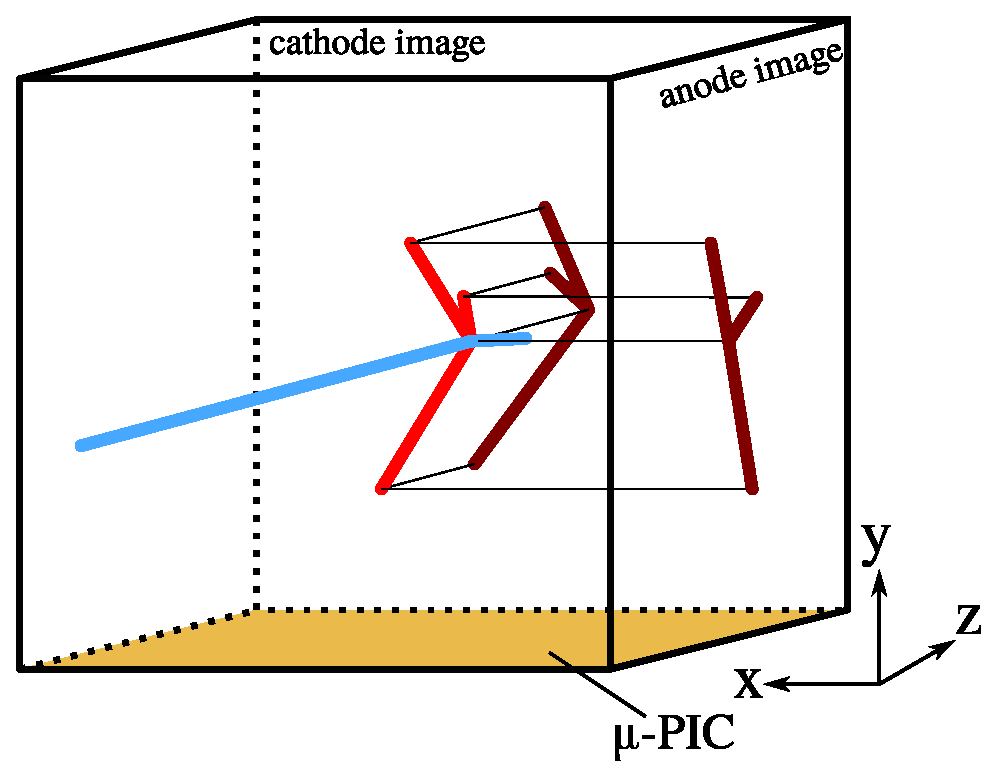
\includegraphics[clip, width=0.7\columnwidth]{eps/MAIKo2.eps}
  \caption[MAIKo TPC の概観図。]{MAIKo TPC の概観図。
    図では紙面手前から入射した中性子 (青) がTPCの中の${}^{12}{\rm C}$と散乱して3つの$\alpha$粒子 (赤) に崩壊した事象を表す。
    anode image ($zy$平面) と cathode image ($zy$平面) の2平面に荷電粒子のトラックが射影される。
    中性子は電荷を持たないためanode \& cathode image にトラックとして検出されない。
  }
  \label{fig::MAIKo_view}
\end{figure}
\begin{figure}
  \centering
%  \includegraphics[clip, width=0.7\columnwidth]{}
  \caption[MAIKo TPC の概観。]{MAIKo TPC の概観。}
  \label{pic::MAIKo}
\end{figure}
MAIKo TPC では3次元のトラックを図\ref{fig::MAIKo_view}のように2つの平面 ($zy, xy$平面) に射影された画像として取得される。

\subsection{MAIKo TPC の構造}
図\ref{fig::MAIKo_view}にMAIKo TPC の概観図、
図\ref{fig::MAIKo_cage}にMAIKo TPC の構造を示す。
\begin{figure}
  \centering
  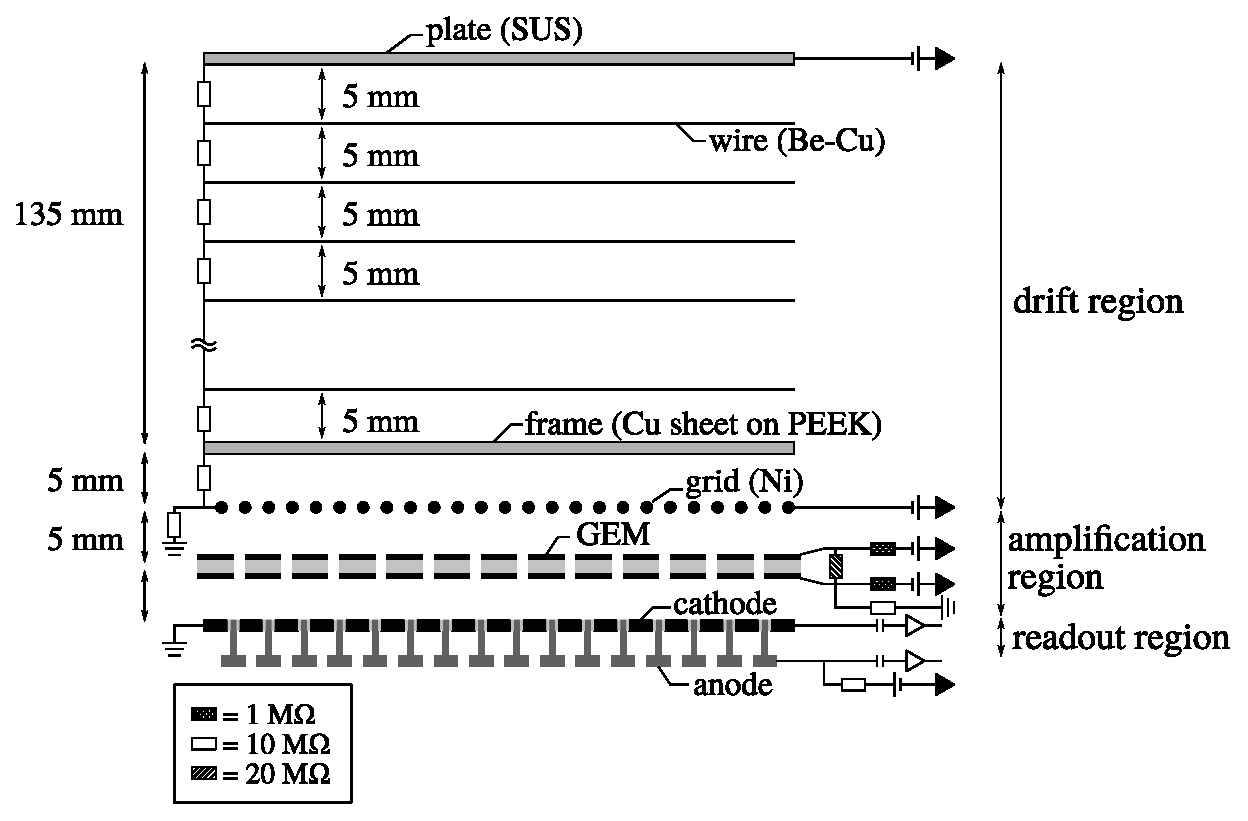
\includegraphics[clip, width=0.9\columnwidth]{eps/MAIKo_cage.eps}
  \caption{MAIKo TPC の構造。}
  \label{fig::MAIKo_cage}
\end{figure}
plate とgrid の間のドリフト領域に電圧をかけることでドリフト電場を形成する。
ドリフト領域を荷電粒子が通過する際に生成された電子が増幅領域へ移動する。
MAIKo TPC ではGEM (gas electron multiplier) と$\mu$-PIC によってドリフト領域からドリフトしてきた電子を増幅する。
増幅した電子およびイオンによって$\mu$-PIC のanode とcathode に誘起される信号を読み出す。

\subsection{ドリフト領域}
plateとwire、grid によって囲まれた領域をドリフト領域と呼ぶ。
grid からplate の方向 (図\ref{fig::MAIKo_cage}では上向き) にドリフト電場を作ることで
荷電粒子の周りに発生した電子を増幅領域へドリフトさせる。
ドリフト電場の一様性が高いほど、電子を均等にドリフトすることができる。
ドリフト電場を一様に形成するためにwire が5 mm 間隔で巻かれている。
plate とgrid のそれぞれに高電圧をかけることによってドリフト電場を調整する。

\subsection{GEM}
$\mu$-PIC にも増幅機構があるが、より大きく増幅するためにGEM を用いた増幅機構を設けている。
GEM は、図\ref{pic::GEM}のようにポリマーのフルムの表面を銅で被覆し、
直径70 $\mu$m の穴を140 $\mu$m 間隔で1 mm$^2$あたり100 個の密度で開けたものである。
銅の2つの層はポリマーによって絶縁されている。
銅の両面に電圧を印加することによって、高電場が形成されてドリフトしてきた種電子が増幅される。
\begin{figure}
  \centering
  %\includegraphics[clip, width=0.7\colmunwidth]{}
  \caption{GEM の拡大図。}
  \label{pic::GEM}
\end{figure}

\subsection{$\mu$-PIC}
読み出しパッドである$\mu$-PICは図\ref{fig::mupic}のようにanode strip とcathode strip が垂直に配置されている。
anode strip、cathode stripともに400~$\mu$m 間隔で256~chに分割されており、
合計512~chで信号を読み出している。
\begin{figure}
  \centering
  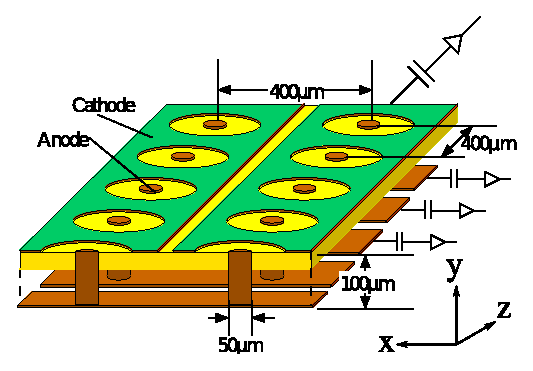
\includegraphics[clip, width=0.7\columnwidth]{eps/upic_struc_xyz.eps}
  \caption[$\mu$-PICの概観図。]{$\mu$-PICの概観図。
    図中の横方向にanode strip、奥行き方向にcathode strip が配置されている。
  }
  \label{fig::mupic}
\end{figure}
図\ref{fig::MAIKo_view}中でanode strip は$z$軸、cathode strip は$x$軸と平行に配置されている。
ドリフト電場により移動してきた電子をanode strip、cathode strip により読み出し、
それぞれ$x$軸、$z$軸座標を検出することができる。
また、anode strip、cathode strip で検出される信号の時間分布により$y$軸座標を決定することができる。

MAIKo TPC からは図\ref{fig::track_demo}のようにanode strip に垂直な面 ($z-y$平面) に射影されたトラックと
cathode strip に垂直な面 ($z-y$平面) に射影されたトラックの2つの画像が出力される。
anode strip とcathode strip はそれぞれ256~chで構成され、
読み出される信号波高の時間変化は100~MHzで1,024~samples測定される。
そのため、出力される画像の解像度は$256\times1,014$~pixels となる。
\begin{figure}
  \centering
  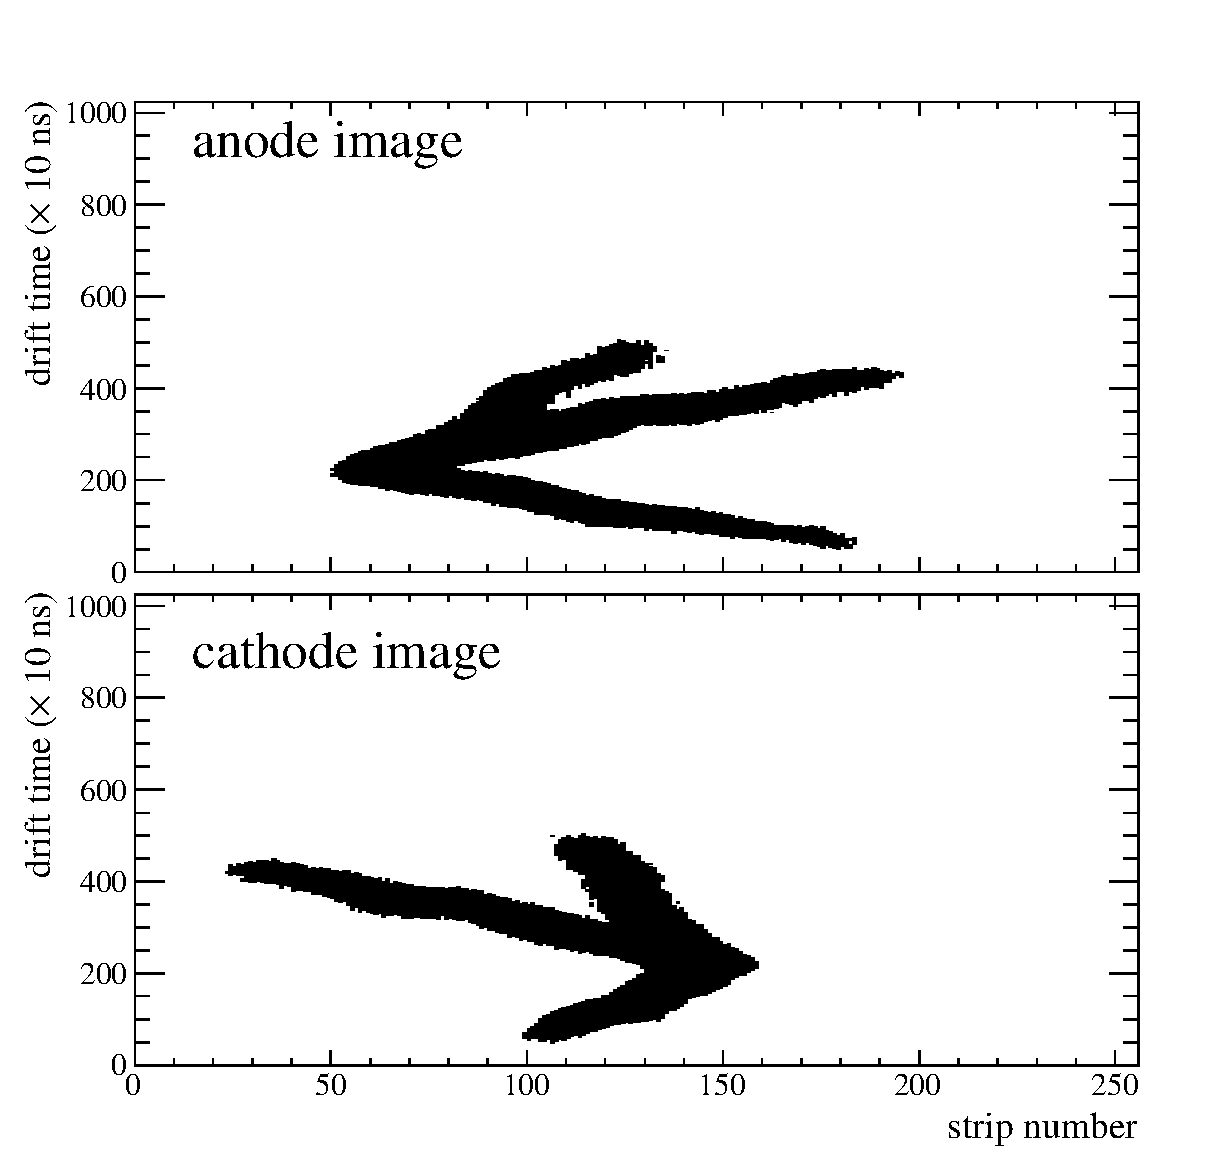
\includegraphics[clip, width=0.7\columnwidth]{eps/10016_6.eps}
  \caption[MAIKo TPC から得られず画像データの一例。]
          {MAIKo TPC から得られず画像データの一例。
          このイベントは\ref{chap::simulation}章で述べるシミュレーションによって生成したデータである。}
  \label{fig::track_demo}
\end{figure}

\section{検出ガスの候補}
標的には炭素の含まれる炭化水素を用いる。
この実験では低エネルギーの荷電粒子のトラックを検出するため、
トラックが比較的長くなるエネルギーロスが小さいガスが適する。
そこで、質量数が最も小さいメタン ($\rm{CH}_{4}$) を用いた。
また、ガスの圧力によってトラックの長さが変化する。
そこで、$\alpha$粒子の検出効率がよくなるガス圧を求めた。

ガス圧はシミュレーションによって決定した。
${}^{12}\rm{C}$と中性子との散乱をKondo らの実験で求められた
微分断面積の角度分布を用いて再現し、
散乱後に${}^{12}\rm{C}$が$Ex = 7.65\rm{MeV}$に励起し、
${}^{12}\rm{C}\rightarrow{}^{8}\rm{Be}+{}^{4}\rm{He}\rightarrow{}^{4}\rm{He}\times 3$
と崩壊する過程を考えた。
この時、$\alpha$粒子が持つエネルギーの分布は図\ref{fig::alphaenergydist}のようになる。
このような粒子に対して
\begin{enumerate}
\item
  MAIKoの有感領域内 ($102.4\rm{mm}\times 102.4\rm{mm}\times 140\rm{mm}$) で停止する
\item
  トラックの長さが$20\rm{mm}$以上である
\end{enumerate}
という条件の時に検出可能とすると、検出効率の圧力依存は図\ref{fig::alphaefficiency}のようになる。
%図\ref{fig::alphaefficiency}より、$75\rm{hPa}$付近が最も検出効率が高いことが分かる。
%そこで、$50\rm{hPa}$、$100\rm{hPa}$の3通りでのオペレートを決定した。

\subsection{ドリフトスピード}
TPCの特性上、ドリフト電場方向の有感領域は電子のドリフト速度に依存する。
ドリフトケージの大きさ ($140\rm{mm}$) を可能な限り使用するためには、
MAIKo TPC のタイムウィンドウ ($10.24\rm{\mu s}$) で$140\rm{mm}$となるようなドリフトスピード
($140\rm{mm}/10.24\rm{\mu s} \sim 0.0135\rm{mm/ns}$) に調整する必要がある。

\subsection{拡散効果}

\subsection{ガスの種類及び圧力の決定}

\section{$\alpha$線源を用いた測定}
\subsection{HV系}
\subsection{ガス系}
\subsection{回路系}
\subsection{電子のドリフト速度}
\subsection{電子の増幅率}

\section{検出ガスの決定}

%ドリフト速度の決定方法は30 degree 方向に$\alpha$線源から$\alpha$を出して、
%その飛跡がデータ上でどう見えるかで決定する。
%ドリフト速度の時間依存性も見た。

%\section{中性子カウンター (液体シンチレータ)}
%\subsection{キャリブレーション}
%\subsection{波形弁別}
%\subsection{検出効率}
%
%\section{中性子カウンター (金属箔)}
%
